\documentclass[12pt]{article}
\usepackage{geometry}
\geometry{a4paper, margin=1in}
\usepackage{graphicx}
\usepackage{titlesec}
\usepackage{xcolor}
\usepackage{hyperref}
\usepackage{fancyhdr}
\usepackage{enumitem}

% Formatting
\titleformat{\section}{\large\bfseries}{\thesection.}{0.5em}{}
\pagestyle{fancy}
\setlength{\headheight}{15pt}
\fancyhf{}
\rhead{EE175A/B - Weekly Progress Report}
\lhead{Battery Management and Communication System}
\rfoot{Page \thepage}

\begin{document}

\begin{center}
    {\Large \textbf{Weekly Progress Report (WPR)}} \\[6pt]
    {\large \textbf{Battery Management and Communication System (BMS)}} \\[2pt]
    \rule{0.8\textwidth}{0.5pt} \\[6pt]
\end{center}

\noindent
\textbf{Team:} Kaushik Vada, Christian Kim, Connor Stewart, Nick Poon \\[3pt]
\textbf{Course:} EE175B - Senior Design II \\
\textbf{Instructor:} Prof. Roman Chomko \\
\textbf{Week:}(\textit{Feb 2 - Feb 8, 2026}) \\[8pt]

\vspace{1em}

\section{Work Completed This Week}
\begin{itemize}[leftmargin=1cm]
    \item Started firmware development by reviewing the schematics to understand the hardware interfaces.
    \item Worked on the core firmware implementation for the Battery Management System (BMS).
    \item Implemented basic firmware interaction with the custom Python GUI to enable real-time monitoring of BMS information.
    \item Designed the BMS firmware architecture to include provisioning for the Electronic Load (E-Load), ensuring seamless integration and real-time GUI connectivity once the E-Load firmware is implemented.
\end{itemize}

\vspace{1em}

\section{Challenges Encountered}
\begin{itemize}[leftmargin=1cm]
    \item Verifying pin mappings between the schematic and the STM32 code to avoid initialization errors, especially with the peripheral pins for the BMS and E-Load.
    \item Establishing a stable serial communication protocol (JSON format) between the firmware and Python GUI initially caused some parsing errors due to buffer overflows.
    \item Ensuring the Python script reliably synchronizes with the data stream upon connection startup to prevent partial packet reads.
\end{itemize}

\vspace{1em}

\section{Work Plan for Next Week}
\begin{itemize}[leftmargin=1cm]
    \item Verify all physical and electrical connections on the BMS board to ensure there are no shorts or soldering issues.
    \item Establish and validate a stable firmware-to-GUI connection.
    \item Ensure a live, real-time data stream is successfully visualized from the BMS to the Python GUI.
\end{itemize}

\vspace{1em}

\section{Appendix A - System Block Diagram}
\begin{center}
    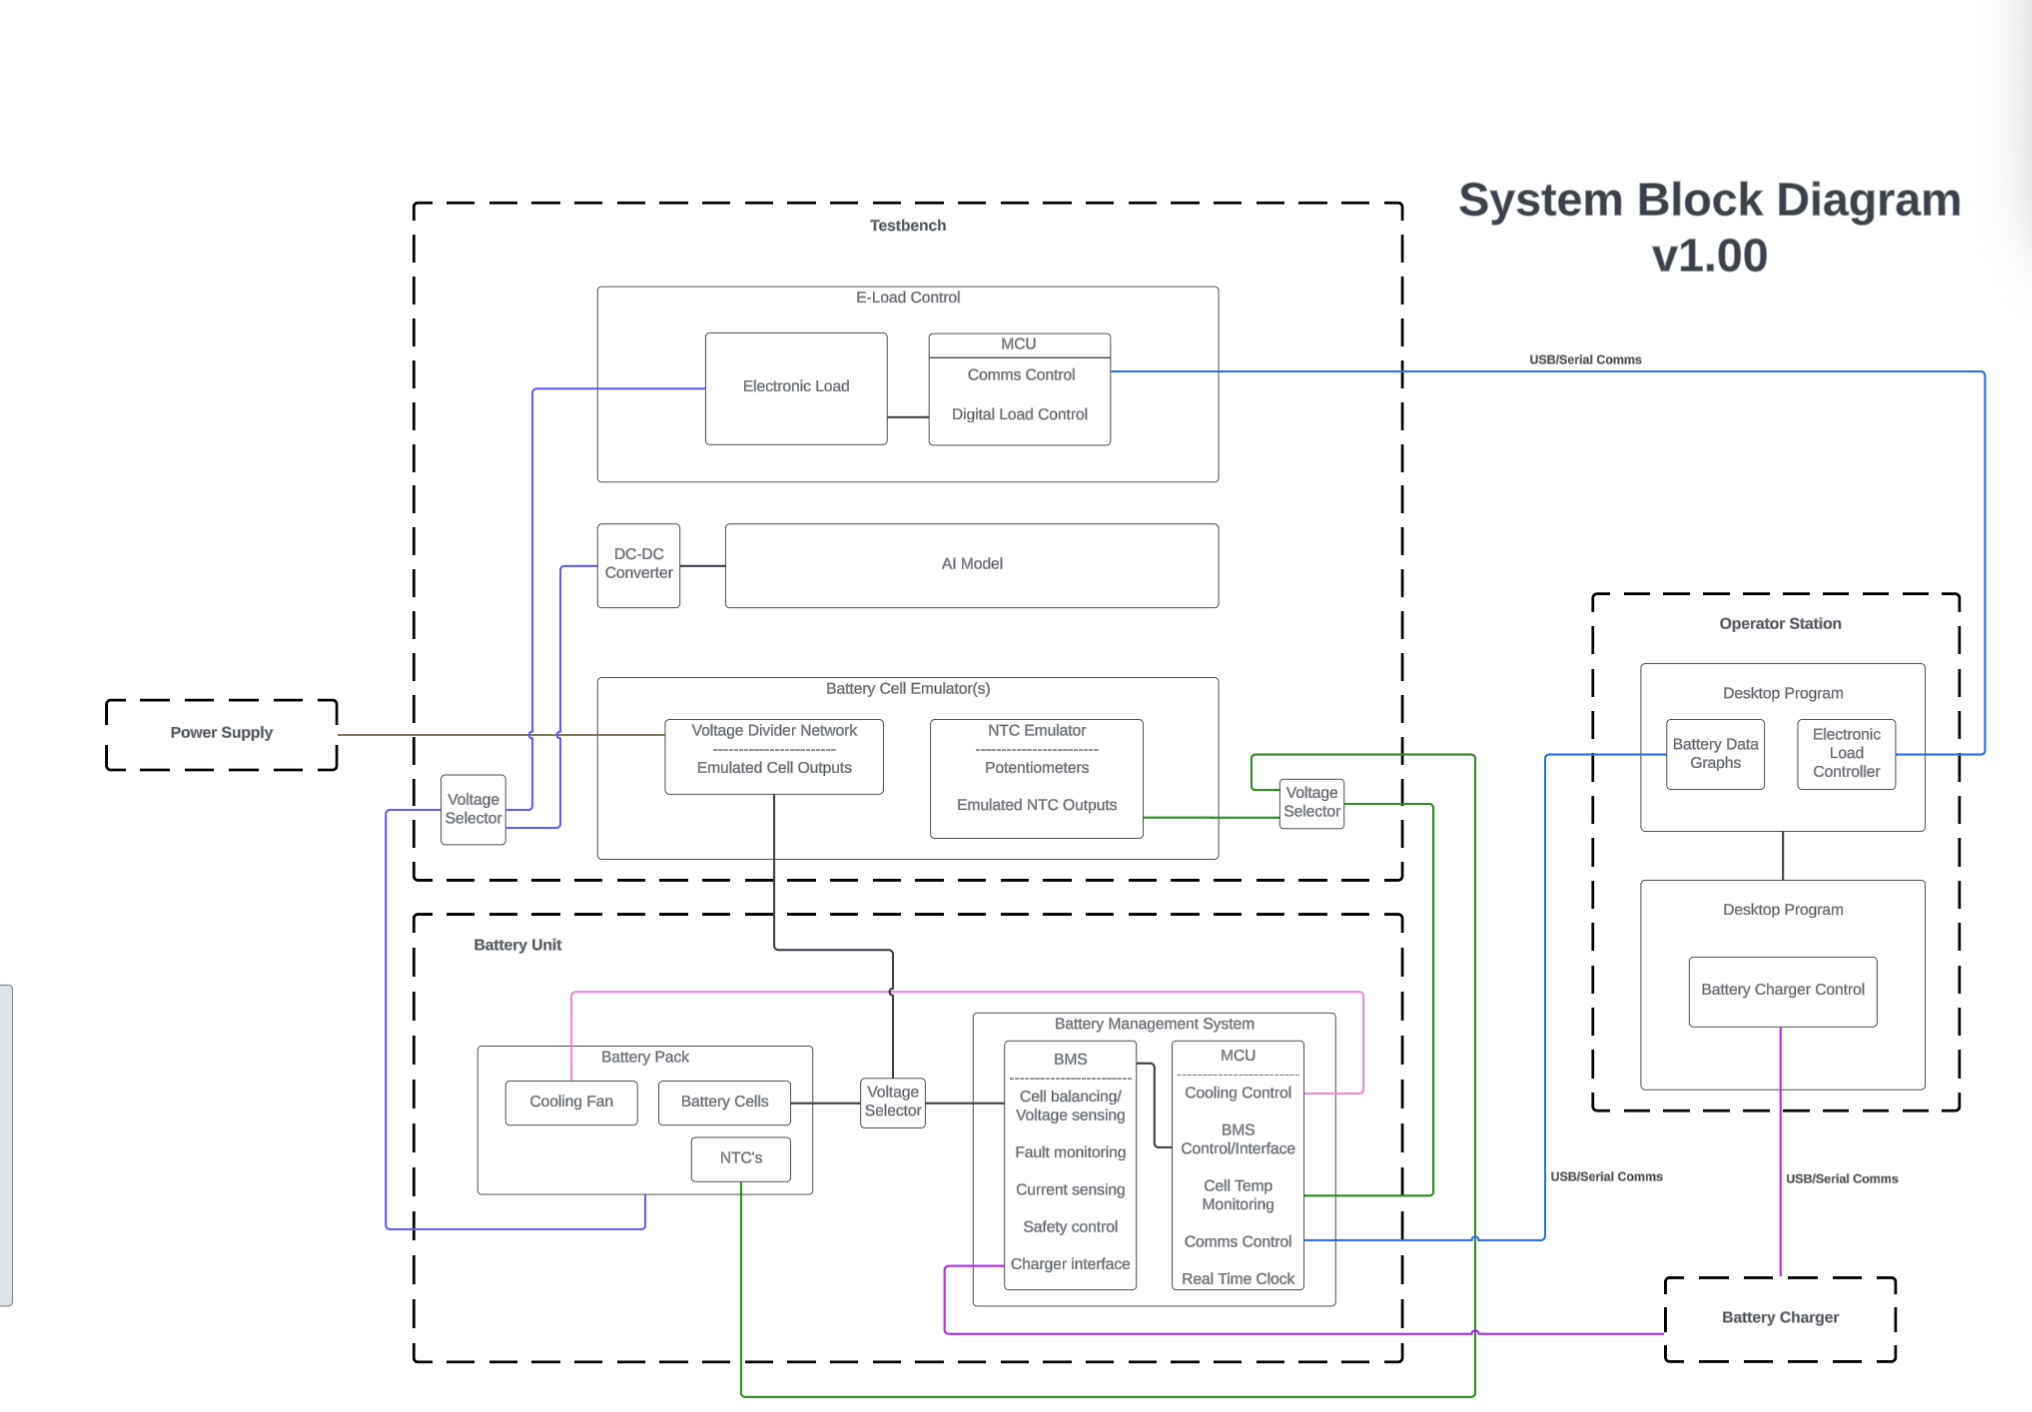
\includegraphics[width=0.95\textwidth]{bms_block_diagram.png} [Figure 1]
\end{center}
\noindent
\textit{Figure A1:} Updated System Block Diagram showing battery domain, isolation components, STM32 communication, and host interface (Source: EE175 Project Report).

\vspace{1em}

\section{Appendix B - Enclosure Visualization}
\begin{center}
    \includegraphics[width=0.95\textwidth]{BMS_enclosure.png} [Figure 2]
\end{center}
\noindent
\textit{Figure B1:} 3D rendering of BMS enclosure with semi-transparent lid, showing airflow, fan, USB-C port, and internal component placement.

\vspace{1em}

\section{Appendix C - Battery Pack Implementation}
\begin{center}
    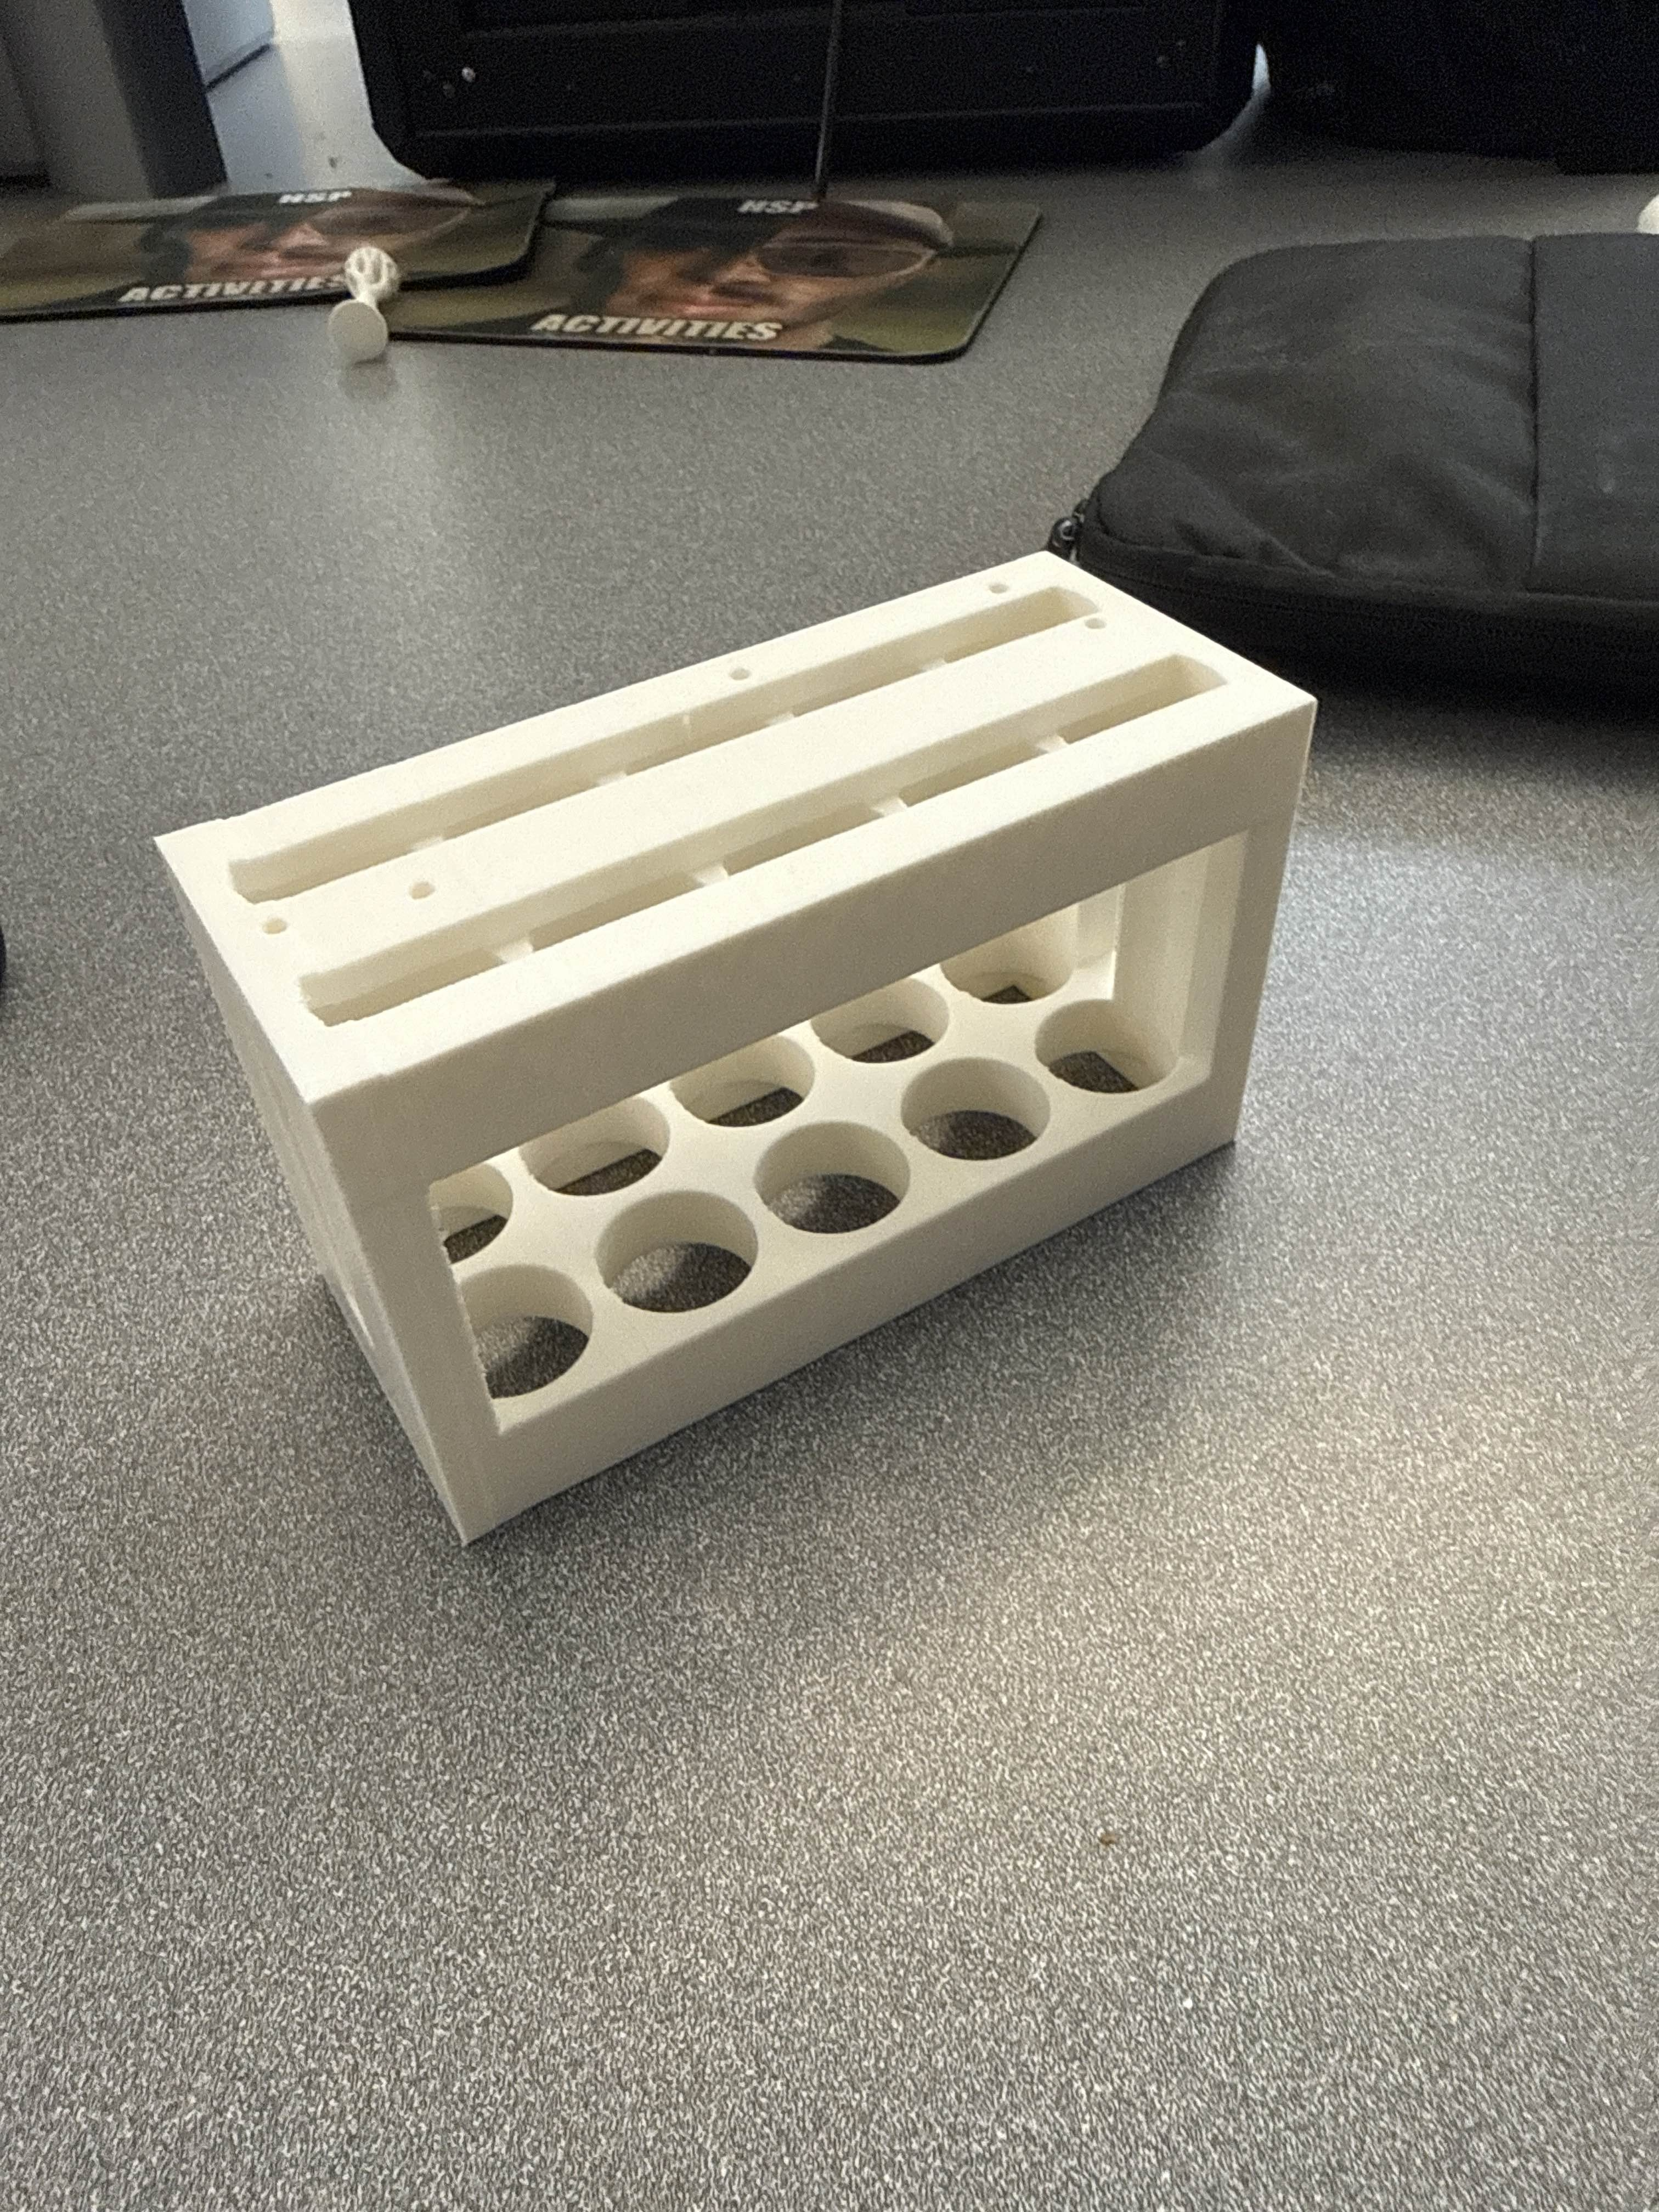
\includegraphics[width=0.95\textwidth]{Battery_Pack.png} [Figure 3]
\end{center}
\noindent
\textit{Figure C1:} Battery pack assembly showing cell arrangement and integration with the BMS unit.

\vspace{1em}

\section{Appendix D - BMS GUI Visualization}
\begin{center}
    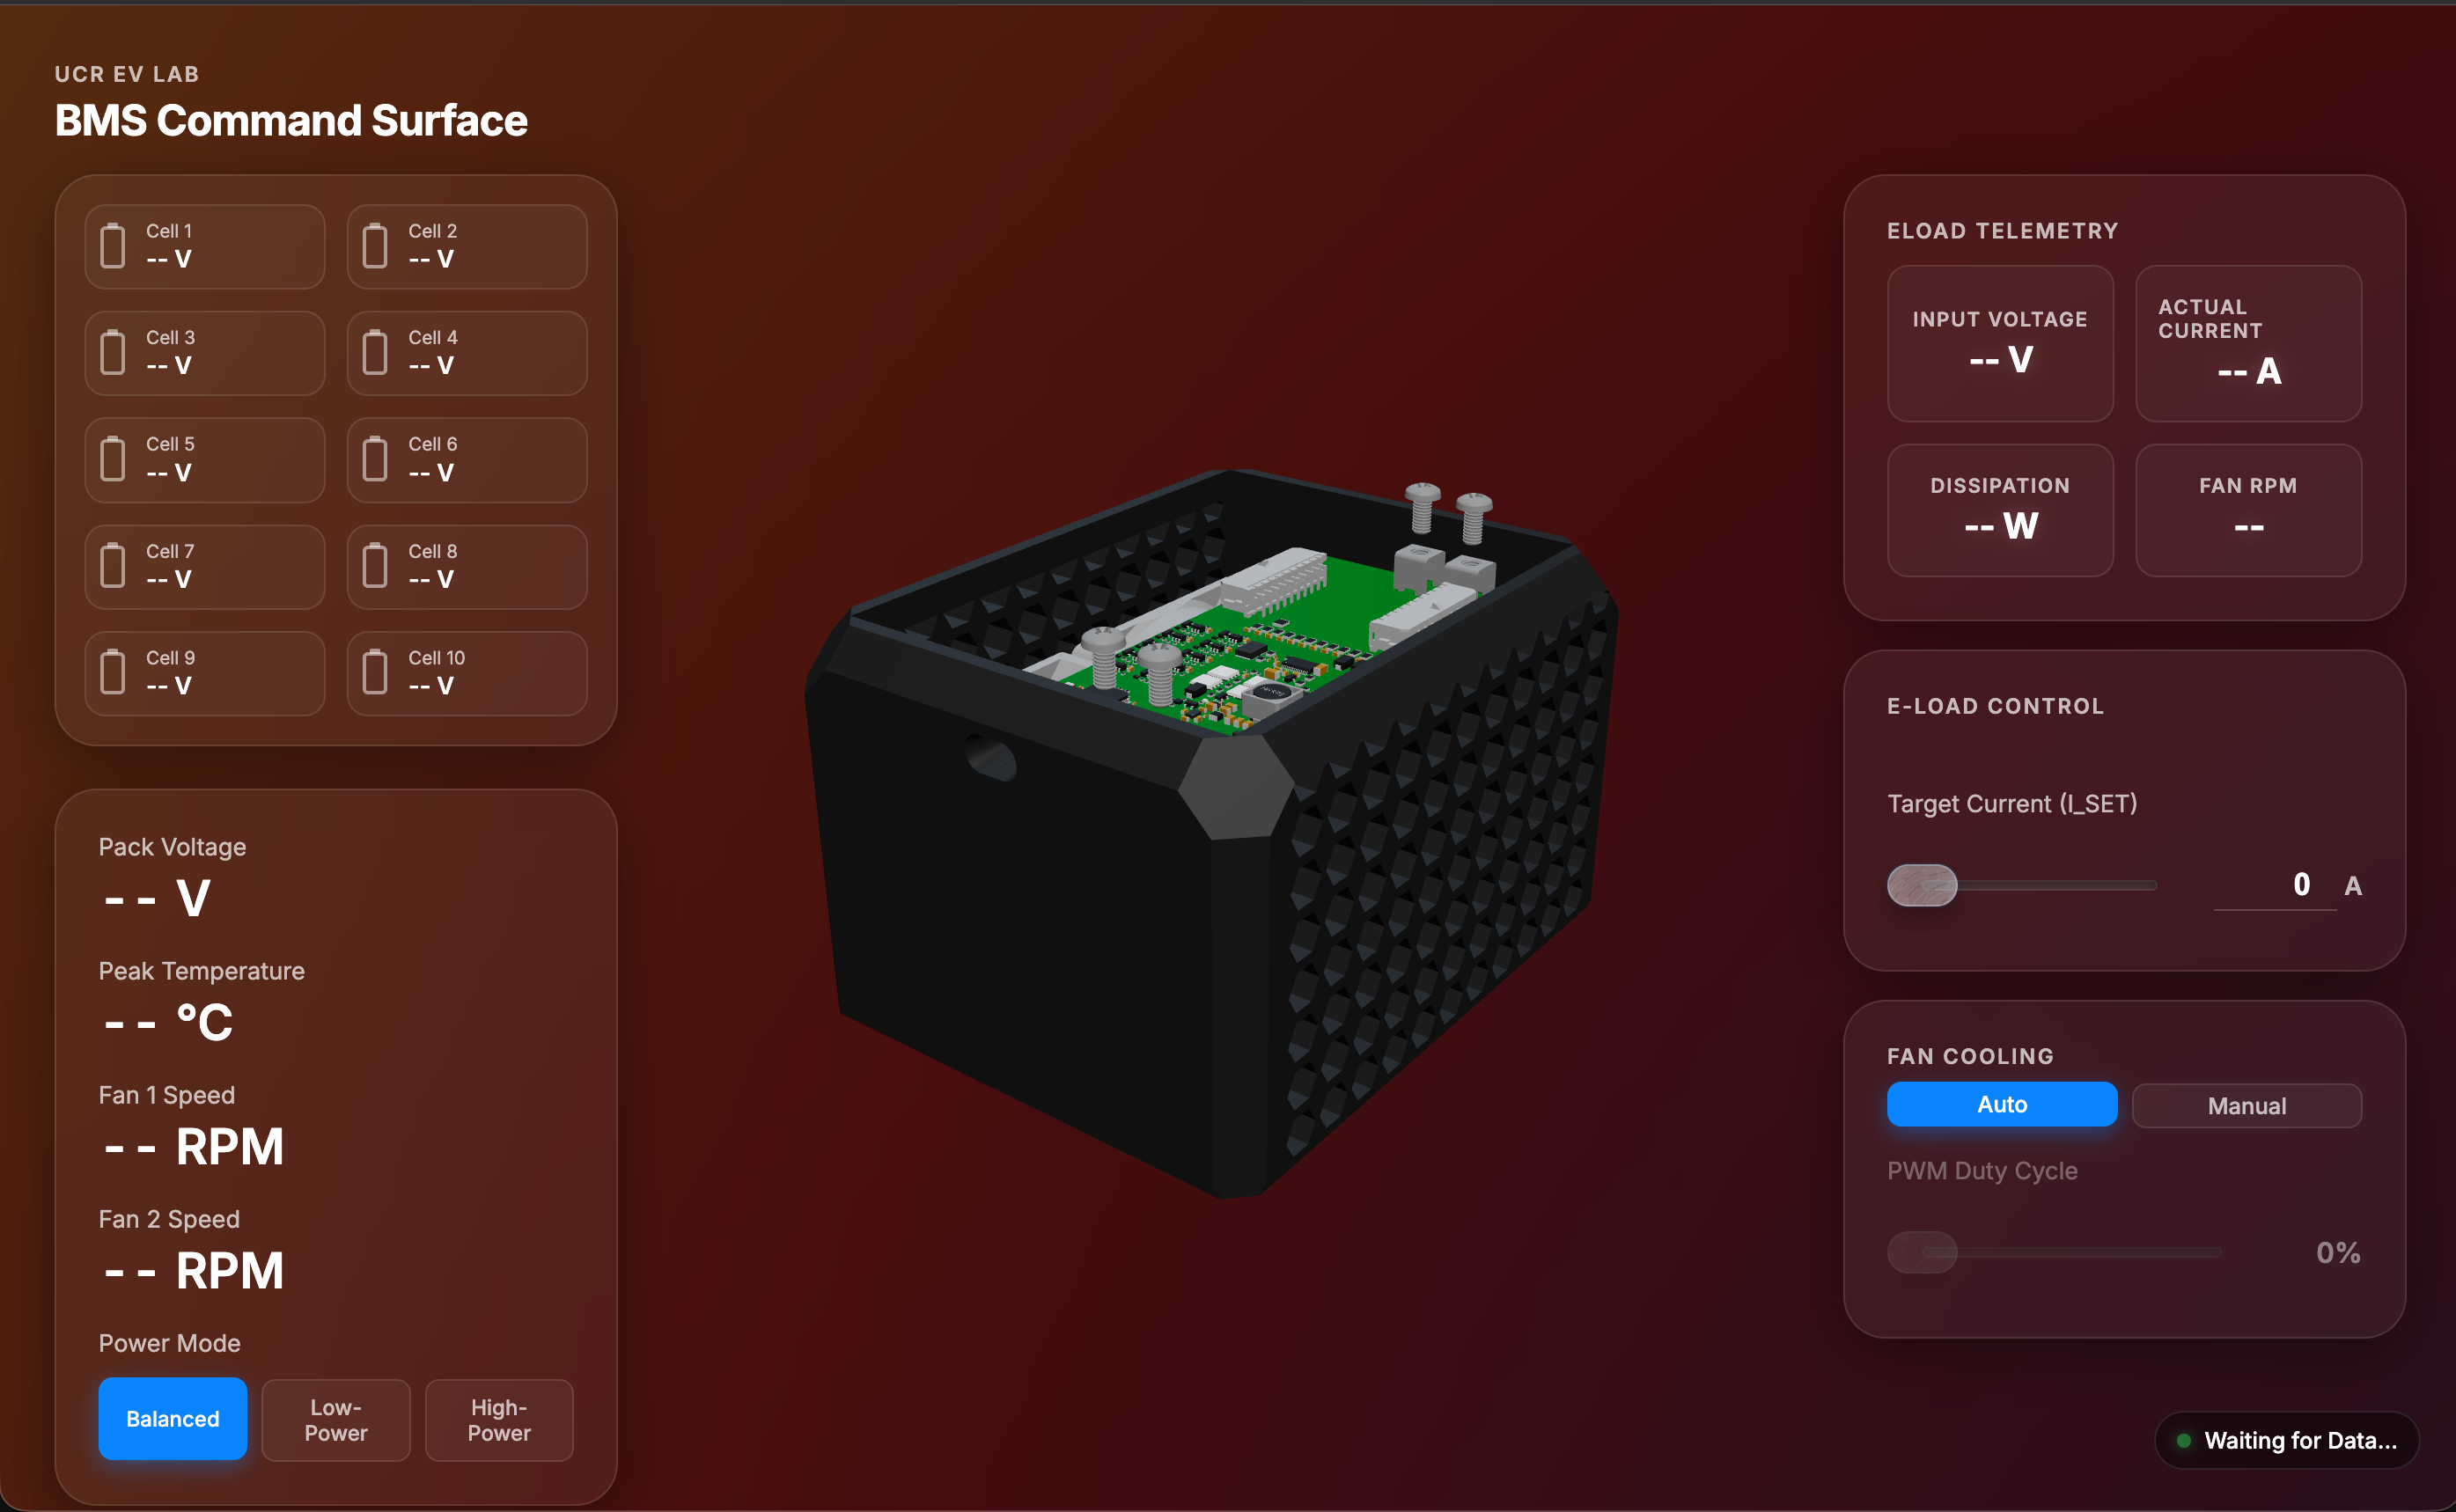
\includegraphics[width=0.95\textwidth]{BMS_GUI.png} [Figure 4]
\end{center}
\noindent
\textit{Figure D1:} Screenshot of the custom Python GUI displaying real-time BMS data, including individual cell voltages, pack voltage, current, and temperature readings.

\end{document}
